% fig_id_stage.tex - id_stage (rtl/id_stage.sv): instruction field slicing,
% control unit (full funct7 + the rs2 field), register file (three read ports,
% the third addressed by rd, + write port driven from WB) and immediate generator.
\documentclass[tikz,border=8pt]{standalone}
\usepackage[T1]{fontenc}
\usepackage{lmodern}
\usepackage[scaled=0.92]{helvet}
\renewcommand{\familydefault}{\sfdefault}
% rv32i_style.tex - shared TikZ styles for the single-cycle RV32I diagrams.
% Visual language:
%   thick border, blue fill  = holds state (clocked)
%   thin border, white fill  = combinational logic
%   green trapezium          = multiplexer (0/1 marks the input chosen by select)
%   dashed orange            = control signal;  solid navy = data
%   /32 on a wire            = bus width;       dot = wires joined
% Port names are the exact SystemVerilog port names of the module drawn.
\usetikzlibrary{arrows.meta, positioning, calc, fit, backgrounds, shapes.geometric, shapes.misc}

\definecolor{ink}{RGB}{31,56,100}
\definecolor{statefill}{RGB}{220,230,242}
\definecolor{muxdraw}{RGB}{56,118,59}
\definecolor{muxfill}{RGB}{226,239,218}
\definecolor{ctrl}{RGB}{197,90,17}
\definecolor{ctrlfill}{RGB}{252,232,216}
\definecolor{note}{RGB}{110,110,110}
\definecolor{tintIF}{RGB}{236,243,251}
\definecolor{tintID}{RGB}{240,247,235}
\definecolor{tintEX}{RGB}{255,246,229}
\definecolor{tintMEM}{RGB}{244,237,249}
\definecolor{tintWB}{RGB}{233,246,245}

\tikzset{
  >={Stealth[length=2.2mm,width=1.6mm]},
  wire/.style      = {draw=ink, line width=0.75pt},
  data/.style      = {wire, ->},
  ctl/.style       = {draw=ctrl, line width=0.75pt, dashed, dash pattern=on 3pt off 1.6pt, ->},
  ctlnoarrow/.style= {draw=ctrl, line width=0.75pt, dashed, dash pattern=on 3pt off 1.6pt},
  block/.style     = {draw=ink, line width=0.75pt, fill=white, rectangle, align=center,
                      inner sep=3pt, font=\small},
  state/.style     = {block, line width=1.8pt, fill=statefill},
  ctrlblock/.style = {block, draw=ctrl, fill=ctrlfill},
  muxst/.style     = {draw=muxdraw, fill=muxfill, line width=0.9pt},
  aluSt/.style     = {draw=ink, fill=white, line width=0.9pt},
  addr/.style      = {circle, draw=ink, fill=white, line width=0.75pt, inner sep=0.5pt,
                      minimum size=6.5mm, font=\large},
  stage/.style     = {draw=ink!70, rounded corners=6pt, line width=0.9pt},
  sig/.style       = {font=\scriptsize\ttfamily, text=ink, inner sep=1.2pt},
  csig/.style      = {font=\scriptsize\ttfamily, text=ctrl, inner sep=1.2pt},
  wlbl/.style      = {font=\tiny, text=ink, inner sep=0.8pt},
  notetxt/.style   = {font=\scriptsize\itshape, text=note, align=left},
  mlbl/.style      = {font=\tiny\bfseries, text=muxdraw, inner sep=0pt},
  title/.style     = {font=\large\bfseries, text=ink},
  dot/.style       = {circle, fill=ink, inner sep=0pt, minimum size=4pt},
  cdot/.style      = {circle, fill=ctrl, inner sep=0pt, minimum size=4pt},
  portbox/.style   = {rectangle, fill=ink, inner sep=0pt, minimum size=4pt},
  cportbox/.style  = {rectangle, fill=ctrl, inner sep=0pt, minimum size=4pt},
  flag/.style      = {sig, draw=ink, fill=white, rounded corners=1.5pt, inner sep=1.5pt},  % net label
  stub/.style      = {ctl},                                                                 % named select input
}

% Two-line block label: module name, then "instance : module".
\newcommand{\blk}[2]{\textbf{#1}\\[-1pt]{\scriptsize\ttfamily #2}}
% Same with a two-line name.
\newcommand{\blkII}[3]{\textbf{#1}\\[-2pt]\textbf{#2}\\[-1pt]{\scriptsize\ttfamily #3}}

% Bus-width mark on a horizontal wire: \wmark{(x,y)}{32}
\newcommand{\wmark}[2]{%
  \draw[draw=ink, line width=0.6pt] ($#1+(-0.07,-0.13)$) -- ($#1+(0.07,0.13)$);
  \node[wlbl, above] at ($#1+(0,0.1)$) {#2};}
% Bus-width mark on a vertical wire: \wmarkv{(x,y)}{32}
\newcommand{\wmarkv}[2]{%
  \draw[draw=ink, line width=0.6pt] ($#1+(-0.13,-0.07)$) -- ($#1+(0.13,0.07)$);
  \node[wlbl, right] at ($#1+(0.1,0)$) {#2};}

% Multiplexer, inputs on the left, output on the right.
% \muxR{name}{x}{y}{height}: defines (name-out), (name-top), (name-bot), (name-l) (left x).
\newcommand{\muxR}[4]{%
  \draw[muxst] ($(#2,#3)+(-0.28,-#4/2)$) -- ($(#2,#3)+(-0.28,#4/2)$)
               -- ($(#2,#3)+(0.28,#4/2-0.28)$) -- ($(#2,#3)+(0.28,-#4/2+0.28)$) -- cycle;
  \coordinate (#1-out) at ($(#2,#3)+(0.28,0)$);
  \coordinate (#1-top) at ($(#2,#3)+(0,#4/2-0.14)$);
  \coordinate (#1-bot) at ($(#2,#3)+(0,-#4/2+0.14)$);
  \coordinate (#1-l)   at ($(#2,#3)+(-0.28,0)$);}

% ALU shape (notched trapezium), inputs a (upper) and b (lower) on the left.
% \aluR{name}{x}{y}{height}: defines (name-a), (name-b), (name-out), (name-op) (top edge).
\newcommand{\aluR}[4]{%
  \draw[aluSt] ($(#2,#3)+(-0.65,#4/2)$) -- ($(#2,#3)+(0.65,#4/4)$) -- ($(#2,#3)+(0.65,-#4/4)$)
               -- ($(#2,#3)+(-0.65,-#4/2)$) -- ($(#2,#3)+(-0.65,-0.28)$) -- ($(#2,#3)+(-0.35,0)$)
               -- ($(#2,#3)+(-0.65,0.28)$) -- cycle;
  \coordinate (#1-a)   at ($(#2,#3)+(-0.65,#4*0.3)$);
  \coordinate (#1-b)   at ($(#2,#3)+(-0.65,-#4*0.3)$);
  \coordinate (#1-out) at ($(#2,#3)+(0.65,0)$);
  \coordinate (#1-op)  at ($(#2,#3)+(0,#4*0.375)$);
  \coordinate (#1-c)   at ($(#2,#3)+(0.12,0)$);}

% Ports on a stage boundary. \inport{x}{y}{name}{width}  (label to the left)
% The width may be empty (1-bit port); it is expanded first so \foreach variables work.
\newcommand{\portw}[1]{\edef\pwtmp{#1}\ifx\pwtmp\empty\else\,[\pwtmp]\fi}
\newcommand{\inport}[4]{%
  \node[portbox] at (#1,#2) {};
  \node[sig, anchor=east] at ($(#1,#2)+(-0.12,0)$) {#3\portw{#4}};}
\newcommand{\cinport}[4]{%
  \node[cportbox] at (#1,#2) {};
  \node[csig, anchor=east] at ($(#1,#2)+(-0.12,0)$) {#3\portw{#4}};}
\newcommand{\outport}[4]{%
  \node[portbox] at (#1,#2) {};
  \node[sig, anchor=west] at ($(#1,#2)+(0.12,0)$) {#3\portw{#4}};}
\newcommand{\coutport}[4]{%
  \node[cportbox] at (#1,#2) {};
  \node[csig, anchor=west] at ($(#1,#2)+(0.12,0)$) {#3\portw{#4}};}
% Control input port on the top edge (label above).
\newcommand{\ctopport}[4]{%
  \node[cportbox] at (#1,#2) {};
  \node[csig, anchor=south] at ($(#1,#2)+(0,0.1)$) {#3\portw{#4}};}
% Data input port on the top edge (label above).
\newcommand{\topport}[4]{%
  \node[portbox] at (#1,#2) {};
  \node[sig, anchor=south] at ($(#1,#2)+(0,0.1)$) {#3\portw{#4}};}

% Legend strip. \legend{x}{y}
\newcommand{\legend}[2]{%
  \begin{scope}[shift={(#1,#2)}, font=\scriptsize]
    \node[state, minimum width=6mm, minimum height=3.5mm, inner sep=0pt] at (0,0) {};
    \node[anchor=west] at (0.45,0) {holds state};
    \node[block, minimum width=6mm, minimum height=3.5mm, inner sep=0pt] at (3.2,0) {};
    \node[anchor=west] at (3.65,0) {combinational};
    \draw[muxst] (6.2,-0.25) -- (6.2,0.25) -- (6.5,0.1) -- (6.5,-0.1) -- cycle;
    \node[anchor=west] at (6.6,0) {multiplexer};
    \draw[data] (8.7,0) -- (9.4,0); \node[anchor=west] at (9.45,0) {data};
    \draw[ctl] (10.4,0) -- (11.1,0); \node[anchor=west] at (11.15,0) {control};
    \node[portbox] at (12.6,0) {}; \node[anchor=west] at (12.7,0) {module port};
    \draw[wire] (14.6,0) -- (15.3,0); \draw[draw=ink, line width=0.6pt] (14.88,-0.13) -- (15.02,0.13);
    \node[wlbl] at (14.95,0.24) {32}; \node[anchor=west] at (15.35,0) {bus width};
  \end{scope}}

\begin{document}
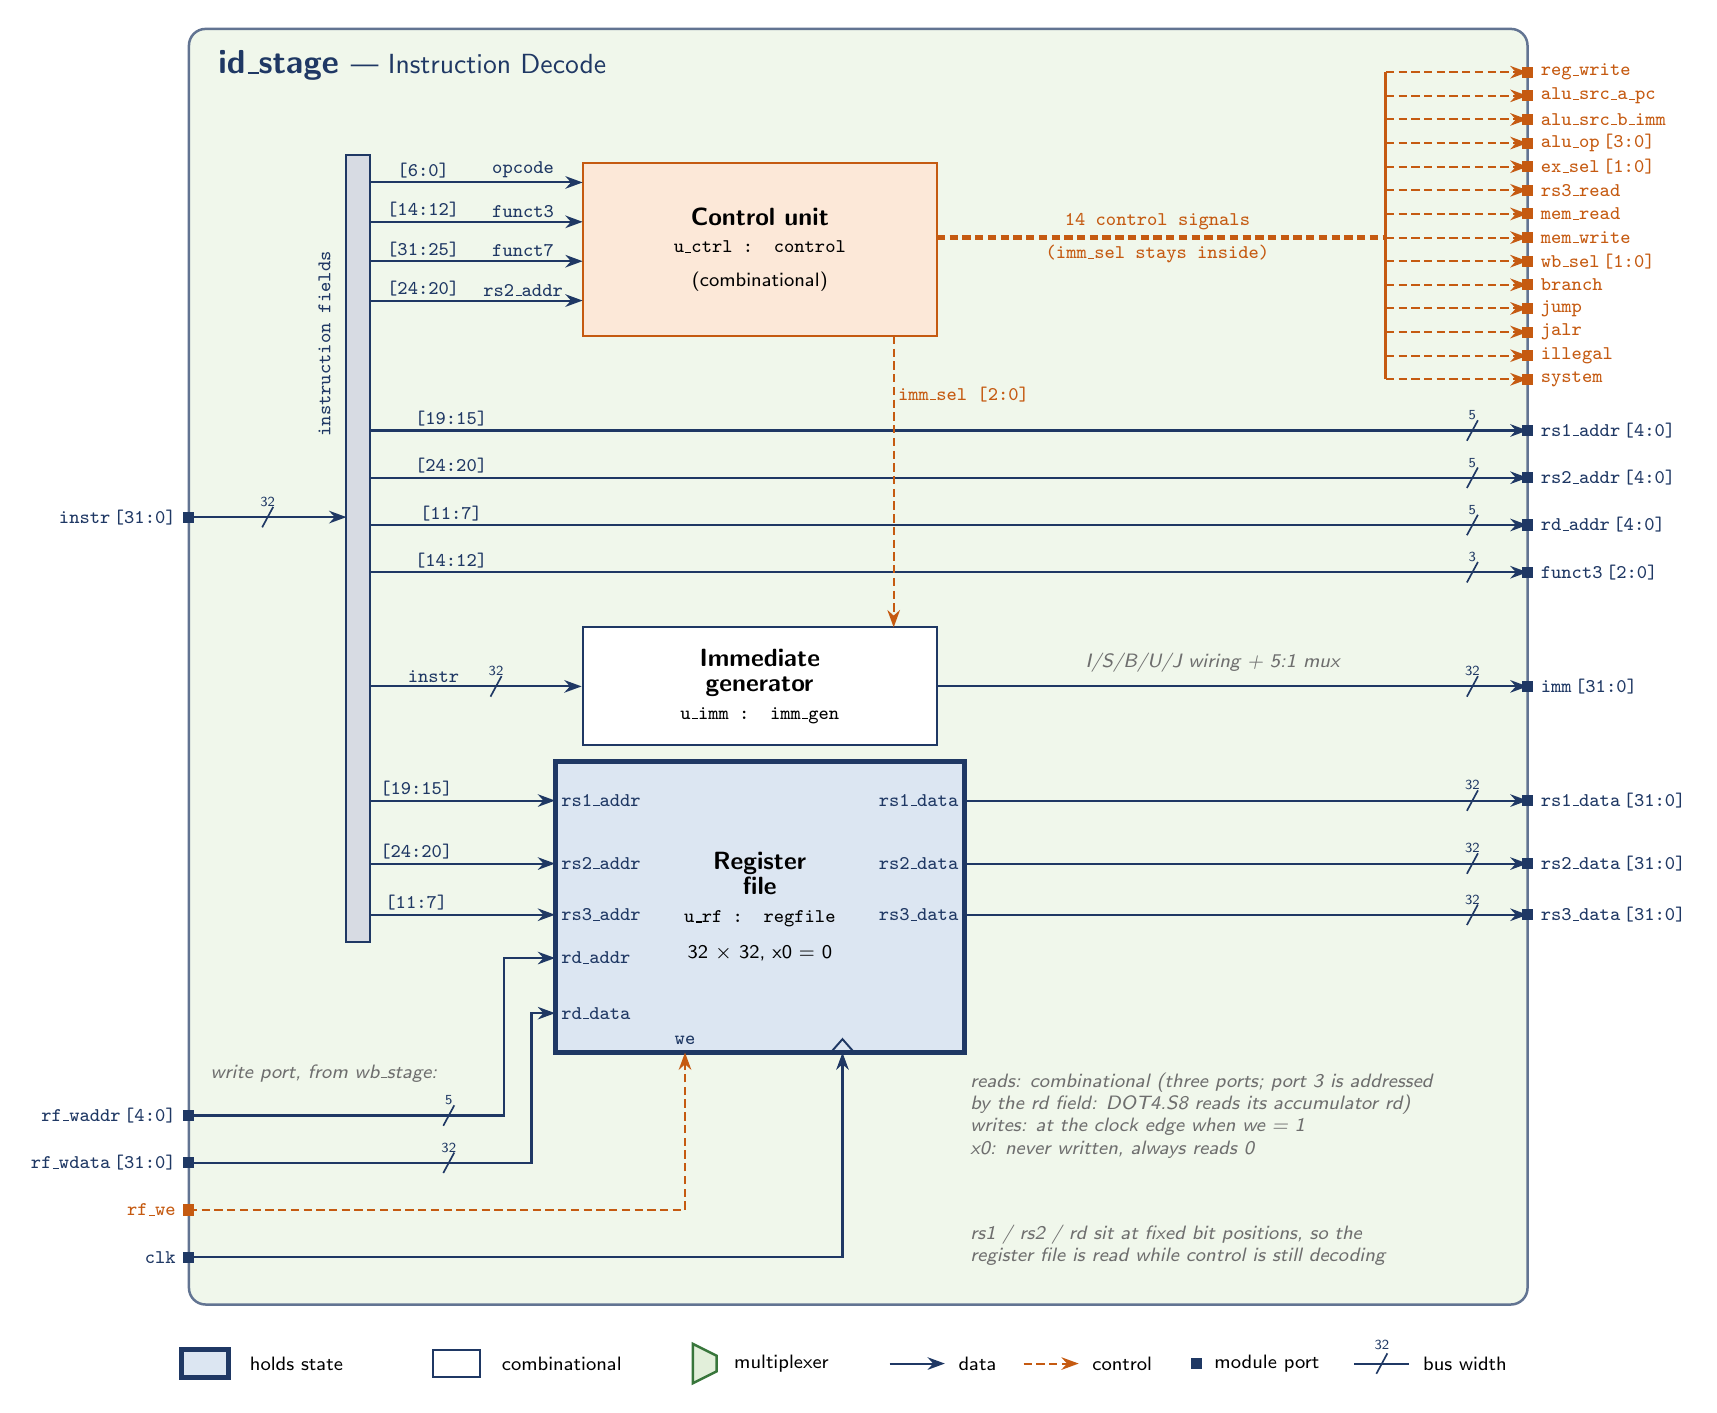
\begin{tikzpicture}
  % ---- stage boundary ----
  \draw[stage, fill=tintID] (0,0) rectangle (17,16.2);
  \node[title, anchor=north west] at (0.25,16.05) {id\_stage \textmd{\normalsize --- Instruction Decode}};

  % ---- input ports ----
  \inport{0}{10.0}{instr}{31:0}
  \inport{0}{2.4}{rf\_waddr}{4:0}
  \inport{0}{1.8}{rf\_wdata}{31:0}
  \cinport{0}{1.2}{rf\_we}{}
  \inport{0}{0.6}{clk}{}
  \node[notetxt, anchor=south west] at (0.15,2.7) {write port, from wb\_stage:};

  % ---- instruction field bus ----
  \draw[draw=ink, fill=ink!18, line width=0.75pt] (2.0,4.6) rectangle (2.3,14.6);
  \node[sig, rotate=90] at (1.72,12.2) {instruction fields};
  \draw[data] (0,10.0) -- (2.0,10.0);
  \wmark{(1.0,10.0)}{32}

  % ---- control unit ----
  \node[ctrlblock, minimum width=45mm, minimum height=22mm] (cu) at (7.25,13.4)
        {\blk{Control unit}{u\_ctrl : control}\\[1pt]{\scriptsize (combinational)}};
  \draw[data] (2.3,14.25) -- node[sig, above, pos=0.25] {[6:0]} node[sig, above, pos=0.72] {opcode} (5.0,14.25);
  \draw[data] (2.3,13.75) -- node[sig, above, pos=0.25] {[14:12]} node[sig, above, pos=0.72] {funct3} (5.0,13.75);
  \draw[data] (2.3,13.25) -- node[sig, above, pos=0.25] {[31:25]} node[sig, above, pos=0.72] {funct7} (5.0,13.25);
  \draw[data] (2.3,12.75) -- node[sig, above, pos=0.25] {[24:20]} node[sig, above, pos=0.72] {rs2\_addr} (5.0,12.75);

  % ---- control outputs: bus, then one port per signal ----
  \draw[ctlnoarrow, line width=1.6pt] (9.5,13.55) -- (15.2,13.55);
  \node[csig, above] at (12.3,13.6) {14 control signals};
  \node[csig, below] at (12.3,13.5) {(imm\_sel stays inside)};
  \draw[draw=ctrl, line width=1.2pt] (15.2,11.75) -- (15.2,15.65);
  \foreach \n/\y/\w in {reg\_write/15.65/, alu\_src\_a\_pc/15.35/, alu\_src\_b\_imm/15.05/,
                         alu\_op/14.75/3:0, ex\_sel/14.45/1:0, rs3\_read/14.15/,
                         mem\_read/13.85/, mem\_write/13.55/,
                         wb\_sel/13.25/1:0, branch/12.95/, jump/12.65/, jalr/12.35/,
                         illegal/12.05/, system/11.75/} {
    \draw[ctl] (15.2,\y) -- (17,\y);
    \coutport{17}{\y}{\n}{\w}
  }

  % ---- decoded fields straight out of the stage ----
  \draw[data] (2.3,11.1) -- node[sig, above, pos=0.07] {[19:15]} (17,11.1);
  \draw[data] (2.3,10.5) -- node[sig, above, pos=0.07] {[24:20]} (17,10.5);
  \draw[data] (2.3,9.9)  -- node[sig, above, pos=0.07] {[11:7]}  (17,9.9);
  \draw[data] (2.3,9.3)  -- node[sig, above, pos=0.07] {[14:12]} (17,9.3);
  \outport{17}{11.1}{rs1\_addr}{4:0}
  \outport{17}{10.5}{rs2\_addr}{4:0}
  \outport{17}{9.9}{rd\_addr}{4:0}
  \outport{17}{9.3}{funct3}{2:0}
  \wmark{(16.3,11.1)}{5}
  \wmark{(16.3,10.5)}{5}
  \wmark{(16.3,9.9)}{5}
  \wmark{(16.3,9.3)}{3}

  % ---- immediate generator ----
  \node[block, minimum width=45mm, minimum height=15mm] (ig) at (7.25,7.85)
        {\blkII{Immediate}{generator}{u\_imm : imm\_gen}};
  \draw[data] (2.3,7.85) -- node[sig, above, pos=0.3] {instr} (ig.west);
  \wmark{(3.9,7.85)}{32}
  \draw[ctl] (8.95,12.3) -- node[csig, right, pos=0.2] {imm\_sel [2:0]} (8.95,8.6);
  \draw[data] (ig.east) -- (17,7.85);
  \outport{17}{7.85}{imm}{31:0}
  \wmark{(16.3,7.85)}{32}
  \node[notetxt, anchor=south] at (13.0,7.9) {I/S/B/U/J wiring + 5:1 mux};

  % ---- register file ----
  \node[state, minimum width=52mm, minimum height=37mm] (rf) at (7.25,5.05)
        {\blkII{Register}{file}{u\_rf : regfile}\\[2pt]{\scriptsize 32 $\times$ 32, x0 = 0}};
  \node[sig, anchor=west] at (4.68,6.4) {rs1\_addr};
  \node[sig, anchor=west] at (4.68,5.6) {rs2\_addr};
  \node[sig, anchor=west] at (4.68,4.95) {rs3\_addr};
  \node[sig, anchor=west] at (4.68,4.4) {rd\_addr};
  \node[sig, anchor=west] at (4.68,3.7) {rd\_data};
  \node[sig, anchor=east] at (9.82,6.4) {rs1\_data};
  \node[sig, anchor=east] at (9.82,5.6) {rs2\_data};
  \node[sig, anchor=east] at (9.82,4.95) {rs3\_data};
  \node[sig, anchor=south] at (6.3,3.25) {we};
  \draw[data] (2.3,6.4) -- node[sig, above, pos=0.25] {[19:15]} (4.65,6.4);
  \draw[data] (2.3,5.6) -- node[sig, above, pos=0.25] {[24:20]} (4.65,5.6);
  \draw[data] (2.3,4.95) -- node[sig, above, pos=0.25] {[11:7]} (4.65,4.95);
  \draw[data] (9.85,6.4) -- (17,6.4);
  \draw[data] (9.85,5.6) -- (17,5.6);
  \draw[data] (9.85,4.95) -- (17,4.95);
  \outport{17}{6.4}{rs1\_data}{31:0}
  \outport{17}{5.6}{rs2\_data}{31:0}
  \outport{17}{4.95}{rs3\_data}{31:0}
  \wmark{(16.3,6.4)}{32}
  \wmark{(16.3,5.6)}{32}
  \wmark{(16.3,4.95)}{32}
  % write port
  \draw[data] (0,2.4) -- (4.0,2.4) -- (4.0,4.4) -- (4.65,4.4);
  \draw[data] (0,1.8) -- (4.35,1.8) -- (4.35,3.7) -- (4.65,3.7);
  \draw[ctl]  (0,1.2) -- (6.3,1.2) -- (6.3,3.2);
  \draw[data] (0,0.6) -- (8.3,0.6) -- (8.3,3.2);
  \draw[ink, line width=0.7pt] (8.15,3.2) -- (8.3,3.37) -- (8.45,3.2);    % clock-input mark
  \wmark{(3.3,2.4)}{5}
  \wmark{(3.3,1.8)}{32}
  \node[notetxt, anchor=west] at (9.8,2.4)
       {reads: combinational (three ports; port 3 is addressed\\by the rd field: DOT4.S8 reads its accumulator rd)\\writes: at the clock edge when we = 1\\x0: never written, always reads 0};
  \node[notetxt, anchor=west] at (9.8,0.75)
       {rs1 / rs2 / rd sit at fixed bit positions, so the\\register file is read while control is still decoding};

  \legend{0.2}{-0.75}
\end{tikzpicture}
\end{document}
